\documentclass[tikz,border=3pt]{standalone}
\usepackage{amsmath}
\usetikzlibrary{arrows.meta,decorations.pathmorphing}

\begin{document}
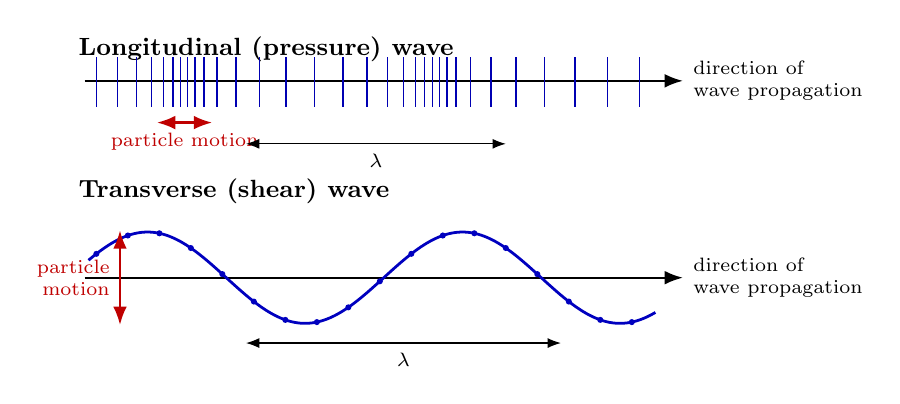
\begin{tikzpicture}[>=Latex,every node/.style={font=\scriptsize}]
  \node[anchor=west,font=\small\bfseries] at (0,3.65) {Longitudinal (pressure) wave};
  \draw[->,line width=.8pt] (0.2,3.25) -- (7.8,3.25)
    node[right,align=left] {direction of\\wave propagation};
  \foreach \x in {0.35,0.62,0.86,1.05,1.20,1.32,1.42,1.51,1.60,1.72,1.88,2.12,2.42,2.76,3.12,3.48,3.79,4.05,4.25,4.40,4.52,4.62,4.71,4.80,4.92,5.10,5.36,5.68,6.04,6.43,6.84,7.25}{
    \draw[blue!70!black,line width=.55pt] (\x,2.92) -- (\x,3.55);
  }
  \draw[<->,red!75!black,line width=.8pt] (1.12,2.72) -- (1.82,2.72)
    node[midway,below] {particle motion};
  \draw[<->] (2.25,2.45) -- node[below] {$\lambda$} (5.55,2.45);

  \node[anchor=west,font=\small\bfseries] at (0,1.85) {Transverse (shear) wave};
  \draw[->,line width=.8pt] (0.2,0.75) -- (7.8,0.75)
    node[right,align=left] {direction of\\wave propagation};
  \draw[blue!75!black,line width=1pt,samples=100,smooth,domain=0.25:7.45,variable=\x]
    plot (\x,{0.75+0.58*sin(90*\x)});
  \foreach \x in {0.35,0.75,...,7.15}{
    \fill[blue!75!black] (\x,{0.75+0.58*sin(90*\x)}) circle (1.1pt);
  }
  \draw[<->,red!75!black,line width=.8pt] (0.65,0.15) -- (0.65,1.35)
    node[midway,left,align=right] {particle\\motion};
  \draw[<->] (2.25,-0.08) -- node[below] {$\lambda$} (6.25,-0.08);
\end{tikzpicture}
\end{document}
